\section{PyLith Application (\protect\object{PyLithApp})}

The top-level object is the PyLith application with three facilities:
\begin{inventory}
  \facilityitem{metadata}{Simulation metadata;}
  \facilityitem{mesher}{Importer for the finite-element mesh;}
  \facilityitem{problem}{Problem to run, such as the materials, boundary conditions, etc.; and}
  \facilityitem{petsc}{PETSc settings.}
\end{inventory}


\subsection{Simulation Metadata (\facility{metadata})}
\newfeature{v3.0.0}

We use metadata to provide a concise summary of a simulation.
The metadata gives structure to information previously placed in comments within the parameter files while also making this information machine readable.
The metadata makes it possible for a Python script to launch an entire suite of simulations and search for simulation parameter files based on the metadata constent (see Section~\vref{sec:runpylith:utilities} for more information).
For example, users can search examples that use a given feature.

At a minumum the metadata must include: (1) a description, (2) the command line arguments necessary to run the simulation, and (3) the PyLith version(s) that are compatible with the input files.
We strongly encourage users to include all of the metadata in their own PyLith parameter files.
\begin{inventory}
  \propertyitem{description}{Description of simulation (required);}
  \propertyitem{authors}{Comma separated list of creator(s) of the simulation;}
  \propertyitem{keywords}{Comma separated list of keywords describing simulation;}
  \propertyitem{features}{Comma separated list of features used in the simulation;}
  \propertyitem{arguments}{Comma separated list of command line arguments for running simulation (required);}
  \propertyitem{base}{Comma separated list of parameter files also containing metadata that complement this metadata;}
  \propertyitem{version}{Version number for simulation; and}
  \propertyitem{pylith\_version}{Command separated list of constraints on the PyLith versions compatible with the parameter files (required)}
\end{inventory}
When using \property{base} to specify other files with metadata, the \property{keywords} and \property{features} will be appended, whereas other metadata will be overwritten (the same behavior as other Pyre properties).

\begin{cfg}[Example of SimulationMetadata in a \filename{.cfg} file.]
<h>[pylithapp.metadata]</h>
<p>base</p> = [pylithapp.cfg]
<p>description</p> = Axial extension using Dirichlet boundary conditions.
<p>keywords</p> = [example, 2D, box, axial extension]
<p>features</p> = [
    Quadrilateral cells,
    pylith.meshio.MeshIOAscii,
    pylith.problems.TimeDependent,
    pylith.materials.Elasticity,
    pylith.materials.IsotropicLinearElasticity,
    spatialdata.spatialdb.UniformDB,
    pylith.meshio.DataWriterHDF5
    ]
<p>authors</p> = [Brad Aagaard]
<p>version</p> = 1.0.0
<p>arguments</p> = [step01_axialdisp.cfg]
<p>pylith_version</p> = [>=3.0, <4.0]
\end{cfg}

\subsection{Mesh Information (\facility{mesher})}

Geometrical and topological information for the finite element mesh
may be provided by exporting an Exodus II format file from
CUBIT/Trelis, by exporting a GMV file and an accompanying Pset file
from LaGriT, or by specifying the information in PyLith mesh ASCII
format. See Chapter \vref{cha:examples} for examples.

PyLith supports linear cells in 2D (Figure \vref{fig:2D:cells}), and
3D (Figure \vref{fig:3D:cells}).  The vertex ordering must follow the
convention shown in Figures \vref{fig:2D:cells}-\vref{fig:3D:cells}.
PyLith no longer supports use of quadratic cells using the PyLith
ASCII mesh format. In the next release, we plan to support higher
order discretizations via PETSc finite-element features from meshes
with linear cells as input.

The mesh information defines the vertex coordinates and specifies
the vertices composing each cell in the mesh. The mesh information
must also define at least one set of vertices for which displacement
(Dirichlet) boundary conditions will be provided. In most realistic
problems, there will be several vertex groups, each with a unique
identifying label. For example, one group might define a surface of
the mesh where displacement (Dirichlet) boundary conditions will be
applied, another might define a surface where traction (Neumann) boundary
conditions will be applied, while a third might specify a surface
that defines a fault. Similarly, the mesh information contains cell
labels that define the material type for each cell in the mesh. For
a mesh with a single material type, there will only be a single label
for every cell in the mesh. See Chapters \vref{cha:material:models}
and \vref{cha:boundary:interface:conditions} for more detailed discussions
of setting the materials and boundary conditions.

\begin{figure}[htbp]
  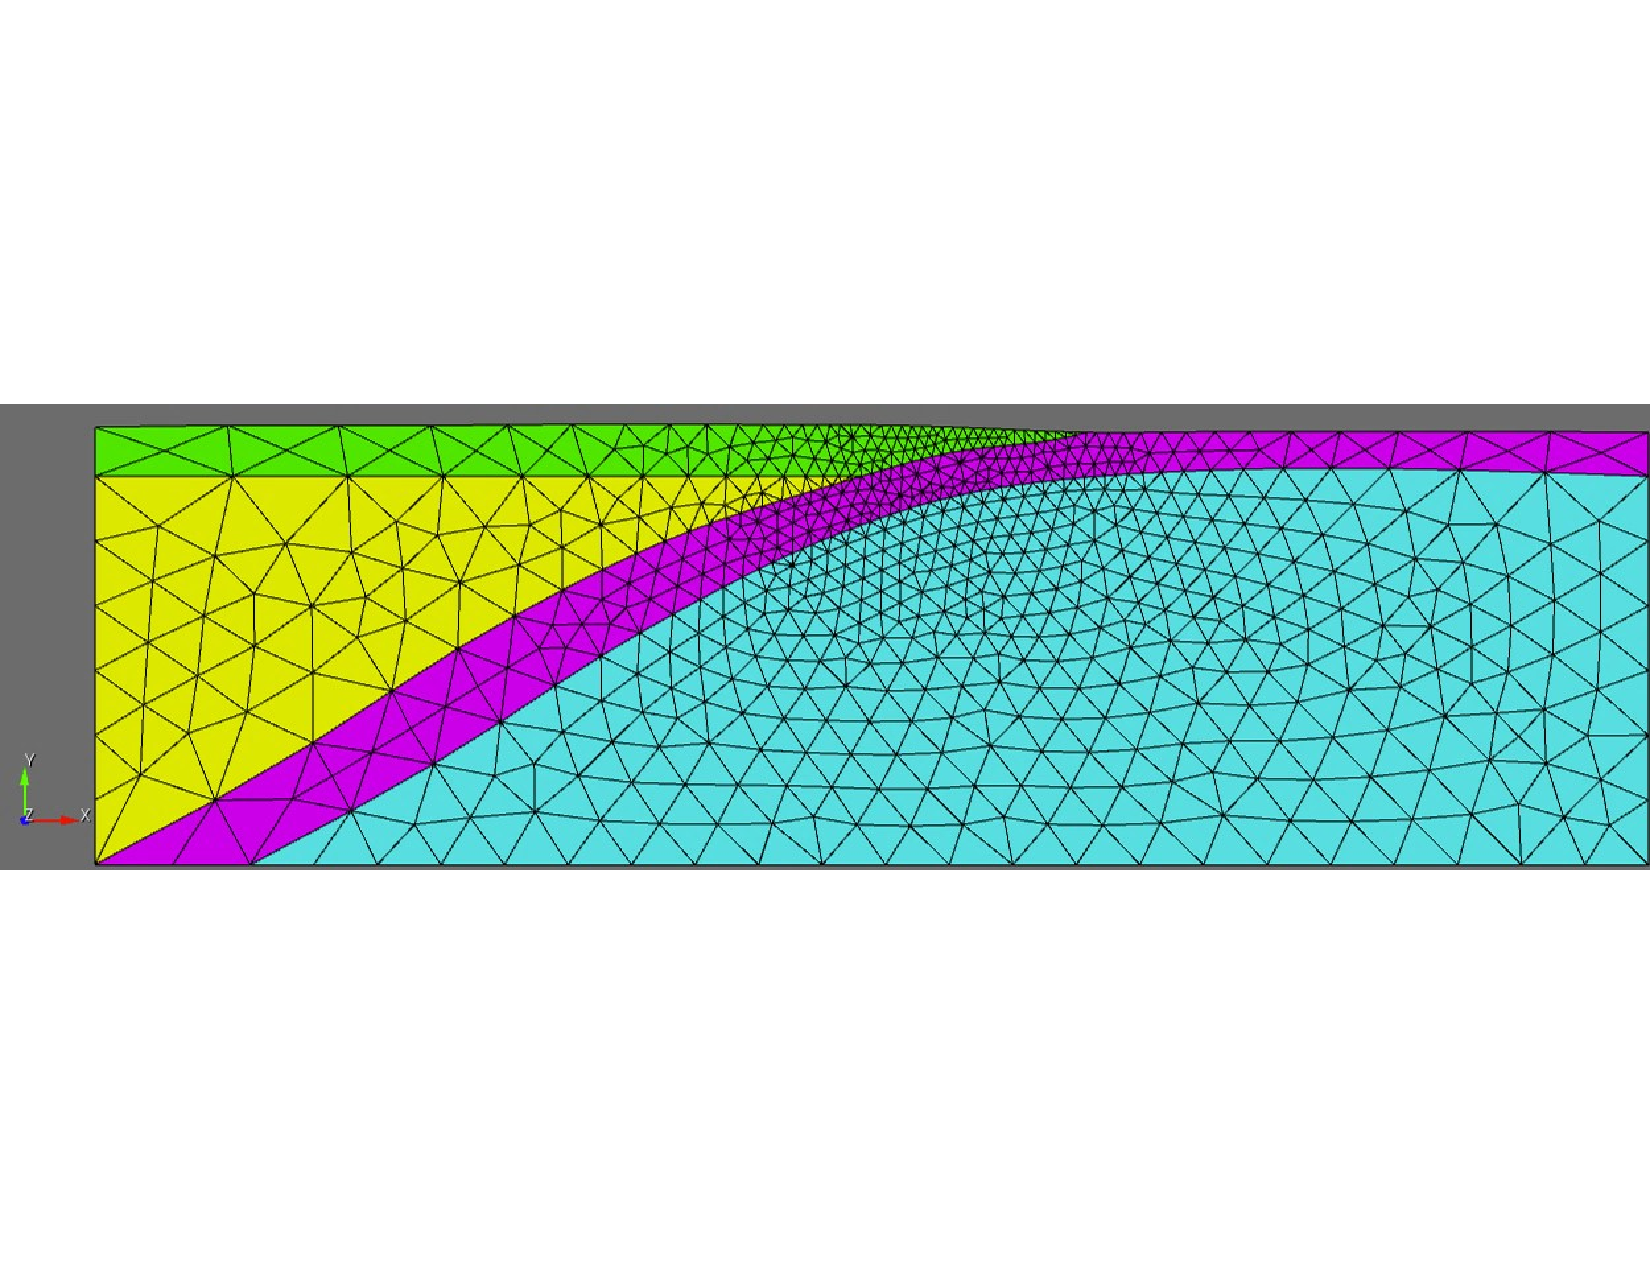
\includegraphics[scale=0.6]{runpylith/figs/tri3}\hspace*{0.5in}%
  \includegraphics[scale=0.6]{runpylith/figs/quad4}
  \caption{Linear cells available for 2D problems are the triangle
    (left) and the quadrilateral (right).}
  \label{fig:2D:cells}
\end{figure}

\begin{figure}[htbp]
  \includegraphics[scale=0.6]{runpylith/figs/tet4}\hspace*{0.5in}%
  \includegraphics[scale=0.6]{runpylith/figs/hex8}
  \caption{Linear cells available for 3D problems are the tetrahedron (left)
    and the hexahedron (right).}
  \label{fig:3D:cells}
\end{figure}

\subsubsection{\object{Mesh Importer}}

The default mesher component is \object{MeshImporter}, which provides
the capabilities of reading the mesh from files. The \object{MeshImporter} has
several properties and facilities:
\begin{inventory}
  \propertyitem{reorder\_mesh}{Reorder the vertices and cells using the
    reverse Cuthill-McKee algorithm (default is False)}
  \facilityitem{reader}{Reader for a given type of mesh (default is
    \object{MeshIOAscii}).}
  \facilityitem{distributor}{Handles
    distribution of the mesh among processors.}
  \facilityitem{refiner}{Perform global uniform mesh refinement after
    distribution among processors (default is no refinement).}
\end{inventory}
Reordering the mesh so that vertices and cells connected topologically
also reside close together in memory improves overall performance
and can improve solver performance as well.

\userwarning{The coordinate system associated with the mesh must be a
  Cartesian coordinate system, such as a generic Cartesian coordinate
  system or a geographic projection.}

\subsubsection{\object{MeshIOAscii}}

The \object{MeshIOAscii} object is intended for reading small, simple
ASCII files containing a mesh constructed by hand. We use this file
format extensively in the examples. Appendix \vref{sec:format:MeshIOAscii}
describes the format of the files. The properties and facilities of
the \object{MeshIOAscii} object include:
\begin{inventory}
\propertyitem{filename}{Name of the mesh file.}
\facilityitem{coordsys}{Coordinate system associated with the mesh.}
\end{inventory}

\subsubsection{\object{MeshIOCubit}}
\label{sec:MeshIOCubit}

The \object{MeshIOCubit} object reads the NetCDF Exodus II files output from
CUBIT/Trelis. Beginning with CUBIT 11.0, the names of the nodesets are included
in the Exodus II files and PyLith can use these nodeset names or revert
to using the nodeset ids. The properties and facilities associated
with the \object{MeshIOCubit} object are:
\begin{inventory}
\propertyitem{filename}{Name of the Exodus II file.}
\propertyitem{use\_nodeset\_names}{Identify nodesets by name rather than id
(default is True).}
\facilityitem{coordsys}{Coordinate system associated with the mesh.}
\end{inventory}

\subsubsection{\object{MeshIOLagrit}}
\label{sec:MeshIOLagrit}

The \object{MeshIOLagrit} object is used to read ASCII and binary GMV and PSET
files output from LaGriT. PyLith will automatically detect whether
the files are ASCII or binary. We attempt to provide support for experimental
64-bit versions of LaGriT via flags indicating whether the FORTRAN
code is using 32-bit or 64-bit integers. The \object{MeshIOLagrit} properties
and facilities are:
\begin{inventory}
  \propertyitem{filename\_gmv}{Name of GMV file.}
  \propertyitem{filename\_pset}{Name of the PSET file.}
  \propertyitem{flip\_endian}{Flip the endian of values when reading
    binary files (default is False).}
  \propertyitem{io\_int32}{Flag
    indicating that PSET files use 32-bit integers (default is True).}
  \propertyitem{record\_header\_32bt}{Flag indicating FORTRAN record header is
    32-bit (default is True).}
\facilityitem{coordsys}{Coordinate system associated with mesh.}
\end{inventory}

\userwarning{The PyLith developers have not used LaGriT since around 2008
  and the most recent release appears to have been in 2010.}

\subsubsection{\object{Distributor}}

The distributor uses a partitioner to compute which cells should be
placed on each processor, computes the overlap among the processors,
and then distributes the mesh among the processors. The type of
partitioner is set via PETSc settings. The properties and facilities
of the \object{Distributor} include:
\begin{inventory}
\propertyitem{partitioner}{Name of mesh partitioner ['chaco','parmetis'].}
\propertyitem{write\_partition}{Flag indicating that the partition information
should be written to a file (default is False).}
\facilityitem{data\_writer}{Writer for partition information (default
  is \object{DataWriterVTK} for VTK output).}
\end{inventory}
\begin{cfg}[\object{Distributor} parameters in a \filename{cfg} file]
<h>[pylithapp.mesh_generator.distributor]</h>
<p>partitioner</p> = chaco ; Options are 'chaco' (default) and 'parmetis'.
\end{cfg}
METIS/ParMETIS are not included in the PyLith binaries due to licensing
issues. 


\subsubsection{\object{Refiner}}

The refiner is used to decrease node spacing by a power of two by
recursively subdividing each cell by a factor of two. In a 2D triangular
mesh a node is inserted at the midpoint of each edge, splitting each
cell into four cells (see Figure \vref{fig:uniform:refinement:2x}).
In a 2D quadrilateral mesh a node is inserted at the midpoint of each
edge and at the centroid of the cell, splitting each cell into four
cells. In a 3D tetrahedral mesh a node is inserted at the midpoint
of each edge, splitting each cell into eight cells. In a 3D hexahedral
mesh a node is inserted at the midpoint of each edge, the centroid
of each face, and at the centroid of the cell, splitting each cell
into eight cells.

\begin{figure}[htbp]
  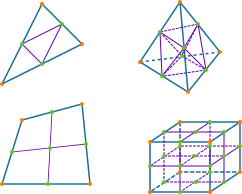
\includegraphics[scale=0.6]{runpylith/figs/refinement2x}
  \caption{Global uniform mesh refinement of 2D and 3D linear
    cells. The blue lines and orange circles identify the edges and
    vertices in the original cells. The purple lines and green circles
    identify the new edges and vertices added to the original cells to
    refine the mesh by a factor of two.}
\label{fig:uniform:refinement:2x}
\end{figure}

Refinement occurs after distribution of the mesh among processors.
This allows one to run much larger simulations by (1) permitting the
mesh generator to construct a mesh with a node spacing larger than
that needed in the simulation and (2) operations performed in serial
during the simulation setup phase, such as, adjusting the topology
to insert cohesive cells and distribution of the mesh among processors
uses this much smaller coarse mesh. For 2D problems the global mesh
refinement increases the maximum problem size by a factor of $4^{n}$,
and for 3D problems it increases the maximum problem size by a factor
of $8^{n}$, where $n$ is the number of recursive refinement levels.
For a tetrahedral mesh, the element quality decreases with refinement
so $n$ should be limited to 1-2.


\subsection{Problem Specification (\protect\facility{problem})}

The problem component specifies the basic parameters of the simulation,
including the physical properties, the boundary conditions, and interface
conditions (faults). The current release of PyLith contains two types
of problems, \object{TimeDependent} for use in static, quasistatic,
and dynamic simulations and \object{GreensFns} for computing static
Green's functions. The general properties facilities include:
\begin{inventory}
  \propertyitem{solver}{Type of solver to use ({\tt linear} or {\tt nonlinear});}
  \facilityitem{solution}{Solution field;}
  \facilityitem{normalizer}{Scales used to nondimensionalize the
    problem (default is \object{NondimElasticQuasistatic});}
  \facilityitem{materials}{Array of materials comprising the domain
    (default is [material]);}
  \facilityitem{bc}{Array of boundary conditions (default is none);}
  \facilityitem{interfaces}{Array of interface conditions, i.e., faults
    (default is none); and}
  \facilityitem{gravity\_field}{Gravity field used to construct body
    forces (default=\object{NullComponent});}
\end{inventory}

\begin{cfg}[Problem parameters in a \filename{cfg} file]
<h>[pylithapp.timedependent]</h>
<p>solver</p> = linear
<f>solution</f> = pylith.problems.SolnDisp
<f>normalizer</f> = spatialdata.units.NondimElasticQuasistatic
<f>materials</f> = [elastic, viscoelastic]
<f>bc</f> = [boundary_east, boundary_bottom, boundary_west]
<f>interfaces</f> = [SanAndreas, SanJacinto]
<f>gravity_field</f> = spatialdata.spatialdb.GravityField
\end{cfg}

The following sections discuss the \facility{solution} and
\facility{normalizer}. Materials, boundary conditions, and interface
conditions are discussed in Chapter \vref{cha:physics} and the gravity
field spatial database is discussed in Section
\vref{sec:gravity:field}.

\subsubsection{Solution Field (\facility{solution})}

The \facility{solution\_field} specifies the subfields of the solution
field along with their discretization. Table
\vref{tab:solution:containers} shows predefined containers for common
subfield collections. Users can create their own containers if they
add different material formulations.

\important{The order of the subfields within the solution field must
  be consistent between the \object{Solution} field object and the
  point-wise functions. The predefined containers are setup to help
  ensure that this is true.}

\important{When a Lagrange multiplier for fault interfaces is
  included, it should always be the last solution subfield. It is
  special case, because it is discretization only on the cohesive
  cells and not over the entire domain.}

\begin{table}[htbp]
  \caption{Predefined containers for solution subfields.}
  \label{tab:solution:containers}
  \begin{tabular}{lll}
    \toprule
    \thead{Object} & \thead{Subfields} & \thead{Use Cases} \\
    \midrule
    \object{SolnDisp} & displacement & Elasticity w/o inertia and faults \\
    \object{SolnDispVel} & displacement, velocity & Elasticity w/inertia and w/o faults \\
    \object{SolnDispLagrange} & displacement, lagrange\_fault & Elasticity w/faults \\
    \object{SolnDispVelLagrange} & displacement, lagrange\_fault & Elasticity w/faults \\
    \object{SolnDispPres} & displacement, pressure & Incompressible elasticity w/o faults \\
    \object{SolnDispPresLagrange} & displacement, pressure, lagrange\_fault & Incompressible elasticity w/o faults \\
    \bottomrule
  \end{tabular}
\end{table}

Each subfield is a \object{SolutionSubfield} object with the following properties:
\begin{inventory}
  \propertyitem{alias}{User-specified name for subfield to use in
    output (default is the PyLith-specified name);}
  \propertyitem{basis\_order}{Order for basis functions (default=1);}
  \propertyitem{quadrature\_order}{Order of quadrature to use in
    integration (default=1);}
  \propertyitem{dimension}{Topological dimension
    associated with subfield (default=-1 and should not be
    changed); and}
  \propertyitem{finite\_element\_space}{Finite-element space ({\tt
      polynomial} or {\tt point; defaults=polynomial}). Point space corresponds to delta
    functions at the quadrature points;}
\end{inventory}

\begin{cfg}[Setting discretization information for a \object{SolnDispLagrange} component in a \filename{cfg} file]
<h>[pylithapp.problem]</h>
<f>solution</f> = pylith.problems.SolnDispLagrange

<h>[pylithapp.problem.solution.subfields]</h>
<p>displacement.basis_order</p> = 1
<p>displacement.quadrature_order</p> = 1

<p>lagrange_fault.basis_order</p> = 1
<p>lagrange_fault.quadrature_order</p> = 1
\end{cfg}


\subsubsection{Nondimensionalization (\facility{normalizer})}

PyLith rescales all parameters provided by the user so that the
simulation solves the equations using nondimensional quantities.  This
permits application of PyLith to problems across a vast range of
spatial and temporal scales. The scales used to nondimensionalize the
problem are length, pressure, density, and time. PyLith provides two
normalizer objects to make it easy to provide reasonable scales for
the nondimensionalization. The \object{NondimElasticQuasistatic}
normalizer (which is the default) has the following properties:
\begin{inventory}
  \propertyitem{length\_scale}{Distance to nondimensionalize length
    (default is 1.0 km).}
  \propertyitem{shear\_modulus}{Shear modulus to nondimensionalize
    pressure (default is 3.0e+10 Pa).}
  \propertyitem{relaxation\_time}{Relaxation time to
    nondimensionalize time (default is 1.0 year).}
\end{inventory}
\begin{cfg}[\object{NondimElasticQuasistatic} parameters in a \filename{cfg} file]
<h>[pylithapp.timedependent.normalizer]</h>
<p>length_scale</p> = 1.0*km
<p>shear_modulus</p> = 3.0e+10*Pa
<p>relaxation_time</p> = 1.0*yr
\end{cfg}
The \object{NondimElasticDynamic} normalizer has the following
properties:
\begin{inventory}
  \propertyitem{shear\_wave\_speed}{Shear wave speed used to
    nondimensionalize length and pressure (default is 3.0 km/s).}
  \propertyitem{mass\_density}{Mass density to nondimensionalize
    density and pressure (default is 3.0e+3 kg/m$^{3}$).}
  \propertyitem{wave\_period}{Period of seismic waves used to
    nondimensionalize time (default is 1.0 s).}
\end{inventory}
\begin{cfg}[\object{NondimElasticDynamic} parameters in a \filename{cfg} file]
<h>[pylithapp.timedependent.normalizer]</h>
<p>shear_wave_speed</p> = 3.0*km/s
<p>mass_density</p> = 3.0e+3*kg/m**3
<p>wave_period</p> = 1.0*s
\end{cfg}

\important{The default nondimensionalization is reasonable for many
  problems; however, it may be necessary to change the default values
  in some cases. When doing this, keep in mind that the
  nondimensionalization generally applies to the minimum values
  encountered for a problem.  For example, in a quasistatic problem,
  the \property{length\_scale} should be on the order of the minimum
  cell size. Similarly, the \property{relaxation\_time} should be on
  the order of the minimum relaxation time or time scale associated
  with time-dependent boundary and interface conditions.}


\subsubsection{Solution Observers (\facility{solution\_observers})}
\label{sec:solution:observers}

The solution observers get notified of updates to the solution. Table
\vref{solution:observers} lists the current implementations of
solution observers, which are used for output.

\begin{table}[htbp]
  \caption{Solution observers.}
  \label{tab:solution:observers}
  \begin{tabular}{lll}
    \toprule
    \thead{Object} & \thead{Use Cases} \\
    \midrule
    \object{OutputSoln} & Output of the solution over the domain; \\
    \object{OutputSolnBoundary} & Output of the solution over an external boundary \\
    \object{OutputSolnPoints} & Output of the solution at discrete points \\
    \bottomrule
  \end{tabular}
\end{table}

All of the solution observers have the following properties:
\begin{inventory}
  \propertyitem{data\_fields}{List of solution subfields to observer/output (default=all which will output all of the subfields);}
  \facilityitem{writer}{Writer for data (default=\object{DataWriterHDF5});}
  \facilityitem{trigger}{Trigger defining how often output is written (default=\object{OutputTriggerStep}); and}
  \facilityitem{field\_filter}{Filter for output fields (default=\object{FieldFilterNone}).}
\end{inventory}
\object{OutputSolnBoundary} adds a property:
\begin{inventory}
  \propertyitem{label}{Label (name of nodeset/pset) identifier of boundary (required);}
\end{inventory}
See Section \vref{sec:output} for detailed information about the
available components for the \facility{writer}, \facility{trigger},
and \facility{field\_filter} facilities.

\begin{cfg}[Setting \object{OutputSolnBoundary} parameters in a \filename{cfg} file]
<h>[pylithapp.problem.solution_observers.boundary]</h>
<p>label</p> = boundary_groundsurf
<p>writer.filename</p> = output/step01-grounssurf.h5
\end{cfg}

\paragraph{Output at Arbitrary Points (\protect\object{OutputSolnPoints})}
\label{sec:output:points}

In many situations with recorded observations, one would like to
extract the solution at the same locations as the recorded
observation. Rather than forcing the finite-element discretization to
be consistent with the observation points, PyLith includes a
specialized solution observer, \object{OutputSolnPoints}, to interpolate
the solution to arbitrary points. The locations
are specified in a text file. The \object{OutputSolnPoints}
includes:
\begin{inventory}
  \propertyitem{data\_fields}{List of solution subfields to
    observer/output (default=all which will output all of the
    subfields);}
  \facilityitem{reader}{Reader for points list (default
    is \object{PointsList}); and}
\end{inventory}

\subsubsection{\object{PointsList} Reader}

This object corresponds to a simple text file containing a list of
points (one per line) where output is desired. See \vref{sec:format:PointsList}
for file format specifications. The points are specified in the coordinate
system specified by \object{OutputSolnPoints}. The coordinates will be transformed
into the coordinate system of the mesh prior to interpolation. The
properties available to customize the behavior of \object{PointsList}
are:
\begin{inventory}
\propertyitem{filename}{Names of file containing list of points.}
\propertyitem{comment\_delimiter}{Delimiter at beginning of line to identify
comments (default is \#).}
\propertyitem{value\_delimiter}{Delimiter used to separate values (default is
whitespace).}
\end{inventory}



\subsection{PETSc Settings (\protect\facility{petsc})}
\label{sec:petsc:options}

PyLith relies on PETSc for the finite-element data structures, linear
and nonlinear solvers, and time-stepping algorithms. PETSc has its own
object-oriented interface for specifying runtime options. Instead of
trying to maintain a Pyre interface to all of the PETSc options, we
use a single \facility{petsc} facility to collect all of the PETSc
options and pass them to PETSc.

PETSc time-stepping options are discussed in Section
\vref{sec:problems:timedependent}.

\subsubsection{Monitor/Logging Settings}

Table \vref{tab:pesc:options:monitor} shows the main monitoring
options offered by PETSc. Our recommended settings for all simulations
include:
\begin{cfg}[Recommended PETSc monitoring settings as set in a \filename{cfg} file.]
<h>[pylithapp.petsc]</h>
# Trigger errors if linear or nonlinear solver fails to converge.
<p>ksp_error_if_not_converged</p> = true
<p>snes_error_if_not_converged</p> = true

# Monitor converged reasons
<p>ksp_converged_reason</p> = true
<p>snes_converged_reason</p> = true

# Monitor time-stepping and nonlinear solver
<p>ts_monitor</p> = true
<p>snes_monitor</p> = true
<p>snes_linesearch_monitor</p> = true
\end{cfg}
When optimizing and troubleshooting solver settings, we usually turn on all the monitoring.

\begin{table}[htbp]
  \caption{Description of PETSc monitoring settings.}
  \label{tab:petsc:options:monitor}
  \begin{tabular}{lp{4.0in}}
    \toprule
    \thead{Option} & \thead{Description} \\
    \midrule
% log
    \property{log\_view} & Show logging objects and events. \\

% TS
    \property{ts\_monitor} & Show time-stepping progress. \\
% KSP
    \property{ksp\_monitor} & Show preconditioned residual norm. \\
    \property{ksp\_view} & Show linear solver parameters. \\
    \property{ksp\_error\_if\_not\_converged} & Generate an error if linear solver does not converge. \\
    \property{ksp\_converged\_reason} & Indicate why iterating stopped in linear solve. \\
% SNES
    \property{snes\_monitor} & Show residual norm for each nonlinear solve iteration. \\
    \property{snes\_view} & Show nonlinear solver parameters. \\
    \property{snes\_error\_if\_not\_converged} & Generate an error if nonlinear solver does not converge. \\
    \property{snes\_converged\_reason} & Indicate why iterating stopped in nonlinear solve. \\
    \property{snes\_linesearch\_monitor} & Show line search information in nonlinear solve. \\
    \bottomrule 
  \end{tabular}
\end{table}


\subsubsection{Solver Settings}

For most problems we use the GMRES method from Saad and Schultz for
the linear solver with solver tolerances around 1.0e-10. When running
large problems, we often raise the solver tolerances by one or two
orders of magnitude to reduce runtime while still achieving suitable
accuracy.

See
\href{http://www.mcs.anl.gov/petsc/petsc-as/documentation/linearsolvertable.html}{PETSc
  linear solver table} for a list of PETSc options for linear solvers
and preconditioners.

\usertip{It is important to keep in mind the resolution of the model and
  observations when setting solver tolerances. For example, matching
  observations with an accuracy of 1.0\si{\milli\meter} does not
  require solving the equations to an accuracy of
  0.0001\si{\milli\meter}.}


\begin{table}[htbp]
  \caption{Recommended starting point for PETSc solver tolerances.}
  \label{tab:petsc:options:solver}
  \begin{tabular}{lcp{4.5in}}
    \toprule
    \thead{Property} & \thead{Value} & \thead{Description} \\
    \midrule
% KSP
    \property{ksp\_rtol} & 1.0e-10 & Stop iterating when the preconditioned KSP residual norm has this amount relative to its starting value.\\
    \property{ksp\_atol} & 1.0e-12 & Stop iterating when the preconditioned KSP residual normal is smaller than this value.\\
% SNES
    \property{snes\_rtol} & 1.0e-10 & Stop iterating when the SNES residual norm has this amount relative to its starting value.\\
    \property{snes\_atol} & 1.0e-10 & Stop iterating when the SNES residual normal is smaller than this value.\\
    \bottomrule 
  \end{tabular}
\end{table}

\paragraph{Settings for small problems}

When running small test problems (about 1k or less unknowns) it is very
handy to use a robust preconditioner so that issues related to the boundary
conditions, material parameters, etc. are more obvious. We recommend
using Incomplete (ILU) factorization.

\begin{cfg}[Recommended PETSc solver settings for small problems]
<h>[pylithapp.petsc]</h>
<p>pc_type</p> = ilu
<p>ksp_type</p> = gmres
\end{cfg}

\paragraph{Settings for medium problems}

When running slightly larger problems (about 10k or less unknowns),
the Additive Schwarz Method (ASM) using Incomplete LU (ILU)
factorization preconditioner is usually more efficient.

\begin{cfg}[Recommended PETSc solver settings for medium problems]
<h>[pylithapp.petsc]</h>
<p>pc_type</p> = asm
<p>ksp_type</p> = gmres
\end{cfg}

\paragraph{Efficient settings for elasticity without a fault}

Algebraic multigrid preconditioner usually works very well on
elasticity problems.

\begin{cfg}[Recommended PETSc solver settings for solving elasticity problems without a fault]
<h>[pylithapp.petsc]</h>
<p>pc_type</p> = ml
<p>ksp_type</p> = gmres
\end{cfg}

\important{The ML algebraic multigrid preconditioner is only available
  if you build PETSc with the ML package. These features are included
  in the PyLith binary packages.}

\paragraph{Efficient settings for elasticity with a fault}

The Lagrange multiplier solution subfield introduces a saddle point in
the system of equations, so we use a Schur complement approach. These
settings are available in
\filename{\$PYLITH\_DIR/share/settings/solver\_fault\_exact.cfg}.

\begin{cfg}[Recommended PETSc solver settings for solving elasticity problems with a fault]
<h>[pylithapp.petsc]</h>
<p>pc_type</p> = fieldsplit
<p>pc_use_amat</p> = true
<p>pc_fieldsplit_type</p> = schur
<p>pc_fieldsplit_schur_factorization_type</p> = full
<p>pc_fieldsplit_dm_splits</p> = true
<p>fieldsplit_displacement_ksp_type</p> = preonly
<p>fieldsplit_displacement_pc_type</p> = lu
<p>fieldsplit_lagrange_multiplier_fault_pc_type</p> = jacobi
<p>fieldsplit_lagrange_multiplier_fault_ksp_type</p> = gmres
<p>fieldsplit_lagrange_multiplier_fault_ksp_rtol</p> = 1.0e-11
<p>fieldsplit_lagrange_multiplier_fault_ksp_converged_reason</p> = true
\end{cfg}


\userwarning{The split fields and algebraic multigrid preconditioning
  currently fails in problems with a nonzero null space. This most
  often occurs when a problem contains multiple faults that extend
  through the entire domain and create subdomains without any
  Dirichlet boundary conditions. The current workaround is to use the
  Additive Schwarz preconditioner without split fields.  See Section
  \vref{sec:Troubleshooting} for the error message encountered in this
  situation.}

\paragraph{Efficient settings for incompressible elasticity}

The pressure solution subfield introduces a saddle point in the system
of equations, so we again use a Schur complement approach. This time
we can use algebraic multigrid preconditioning on each block. These
settings are available in
\filename{\$PYLITH\_DIR/share/settings/solver\_incompressible\_elasticity.cfg}.

\begin{cfg}[Recommended PETSc solver settings for solving incompressible elasticity problems without a fault]
<h>[pylithapp.petsc]</h>
<p>pc_type</p> = fieldsplit
<p>pc_fieldsplit_type</p> = schur
<p>pc_fieldsplit_schur_fact_type</p> = full
<p>pc_fieldsplit_schur_precondition</p> = full
<p>fieldsplit_displacement_pc_type</p> = lu
<p>fieldsplit_pressure_pc_type</p> = lu
\end{cfg}


% End of file
